\chapter{\textbf{Queueing Network Solving And BottleNeckAnaliysis}}


For the three classes of jobs obtained, we have set the population of each closed classes of job to 1000 for Startup Sampling Water inland and Outgoing as established in the requirements, and a workload rate of 0.001, which within our requirements indicates 1 / ms, regarding Check Water Quality.
Once parameterized the Queueing Network, the data was inserted into Java Modelling Tool (JMT).\\
Various output Indices were analyzed in first analysis. Performance Indices:
\begin{itemize}
\item Utilization:
	\begin{itemize}
		\item Control Center Server;
		\item SPCU In;
		\item SPCU Out;
		\item Water Company Server;
		\item Purification System;
		\item Water Company Disk.
	\end{itemize}
\item Response Time:
	\begin{itemize}
		\item Control Center Server;
		\item SPCU In;
		\item SPCU Out;
		\item Water Company Server;
		\item Purification System;
		\item Water Company Disk.
	\end{itemize}
\item Response Time Sink (Check Water Quality);
\item Throughput for Sink (Check Water Quality).
\end{itemize}

After the first simulation all the requirements established at the beginning of the work were respected and we did not get any bottoleneck, infact: 
\begin{itemize}
	\item Utilization:
	\begin{itemize}
		\item Control Center Server = 0.0234;
		\item SPCU In = 0.0223;
		\item SPCU Out = 0.0221;
		\item Water Company Server = $ 6.17*10^{-3}$ ;
		\item Purification System = $ 1.13*10^{-3}$;
		\item Water Company Disk = 0.5030.
	\end{itemize}
	\item Response Time:
	\begin{itemize}
		\item Sampling In = 92.0318 us;
		\item Sampling Out = 98.9638.
	\end{itemize}
	\item Response Time Sink (Check Water Quality) = 1183.03576 us;
\end{itemize}

Then we choose to run multiple simulations increasing the number of sensors to understand how the system scales and how it responds to the increasing of inputs. For this purpose we have done a What-If simulation composed of twenty sub-simulation and it has come out that the Utilization performance of the Water Company Disk gets worse when the four thousand sensors are reached.\\
Other proof of this is the analysis of the Response Time.

\begin{center}
  \makebox[\textwidth]{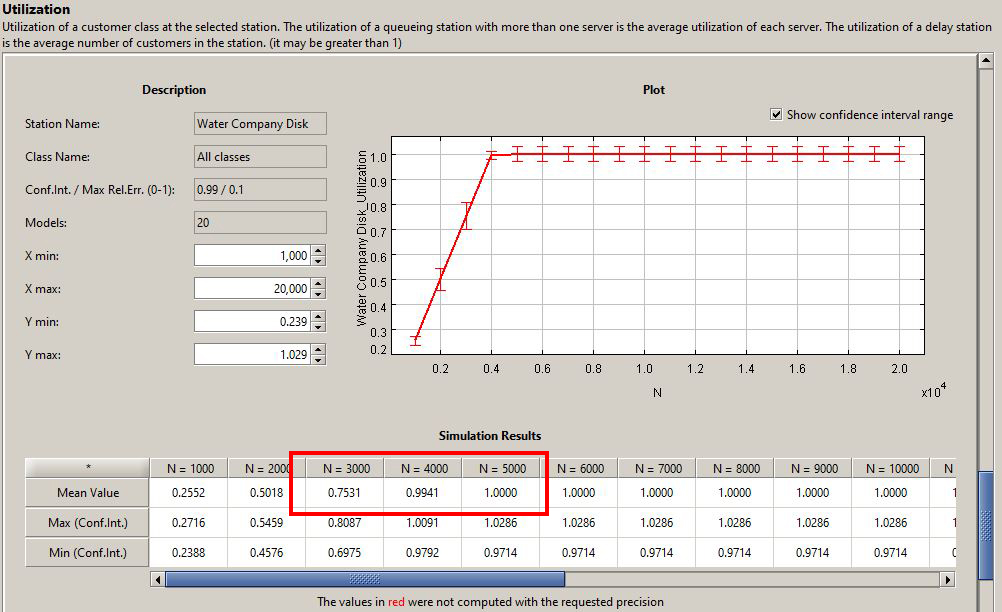
\includegraphics[width=\textwidth]
 {UtilizationWaterCompanyDisk.jpg}}
\end{center}
\captionof{figure}{Water Company Disk Utilization}
\bigskip

Then we choose to run multiple simulations with increasing number of sensors to understand how the system scales and how it
respond to the increasing of inputs. For this purpose we have done a What-If simulation composed of one hundred sub-simulation and it has come out that the Utilization performance of the Water Company Disk gets worse when the fourteen thousand sensors are reached.\\
Other proof of this is the analysis of the Response Time.

\section{Refactoring}

For the refactoring phase we wanted to consider the case in which we want to increase the number of Seaweed Picking to twenty thousand units. in this case, as we saw in the previous analysis, we have a bottleneck linked to the Control Center Server and to the Water Company Disk.

\begin{itemize}
	\item Software Solution;
	\item Hardware Solution.
\end{itemize}

We have chosen a hardware solution because we have decided to have four separate Water Company Disks that translates into a modification of the architecture.\\ %%Mettere i RISULTATI